\chapter{幾何学 - Geometry}

\index{幾何学 - geometry}

幾何学問題は時に複雑で、問題の解を合理的に求め、かつ特殊なケースの数が少なくなるようにアプローチする方法を見つけることは、しばしば困難なことです。

例えば、四辺形(4つの頂点を持つ多角形)の頂点が与えられ、その面積を計算する問題を考えてみましょう。例えば、この問題の入力として、次のようなものがあります。


\begin{center}
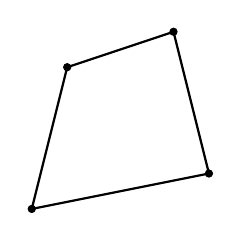
\begin{tikzpicture}[scale=0.45]

\draw[fill] (6,2) circle [radius=0.1];
\draw[fill] (5,6) circle [radius=0.1];
\draw[fill] (2,5) circle [radius=0.1];
\draw[fill] (1,1) circle [radius=0.1];
\draw[thick] (6,2) -- (5,6) -- (2,5) -- (1,1) -- (6,2);
\end{tikzpicture}
\end{center}

この問題へのアプローチの1つは対向する2つの頂点間の直線で2つの三角形に分割することです。

\begin{center}
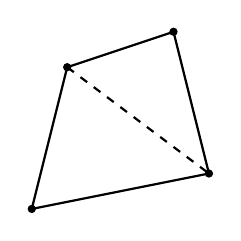
\begin{tikzpicture}[scale=0.45]

\draw[fill] (6,2) circle [radius=0.1];
\draw[fill] (5,6) circle [radius=0.1];
\draw[fill] (2,5) circle [radius=0.1];
\draw[fill] (1,1) circle [radius=0.1];

\draw[thick] (6,2) -- (5,6) -- (2,5) -- (1,1) -- (6,2);
\draw[dashed,thick] (2,5) -- (6,2);
\end{tikzpicture}
\end{center}

あとは、三角形の面積を合計すればよく、三角形の面積は、\key{Heron's formula - ヘロンの公式}で計算できます。
%\footnote{Heron of Alexandria (c. 10--70) was a Greek mathematician.}
\[ \sqrt{s (s-a) (s-b) (s-c)},\]
ここで、$a$,$b$,$c$は三角形の各辺の長さで、
$s=(a+b+c)/2$とします。
\index{ヘロンの公式 - Heron's formula}

これはこれでよいアプローチなのですがひとつ落とし穴があります。
四角形をどうやって三角形に分割するのか。実は任意の2つの対向する頂点を選べない場合があります。
例えば、次のような場合、分割線は四辺形の外に出てしまいますね。

\begin{center}
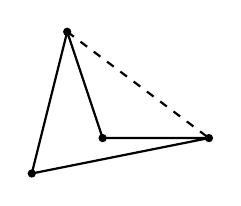
\begin{tikzpicture}[scale=0.45]

\draw[fill] (6,2) circle [radius=0.1];
\draw[fill] (3,2) circle [radius=0.1];
\draw[fill] (2,5) circle [radius=0.1];
\draw[fill] (1,1) circle [radius=0.1];
\draw[thick] (6,2) -- (3,2) -- (2,5) -- (1,1) -- (6,2);

\draw[dashed,thick] (2,5) -- (6,2);
\end{tikzpicture}
\end{center}
ただ、もう一つの線引きの方法は有効です。
\begin{center}
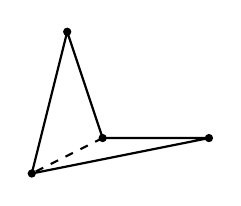
\begin{tikzpicture}[scale=0.45]

\draw[fill] (6,2) circle [radius=0.1];
\draw[fill] (3,2) circle [radius=0.1];
\draw[fill] (2,5) circle [radius=0.1];
\draw[fill] (1,1) circle [radius=0.1];
\draw[thick] (6,2) -- (3,2) -- (2,5) -- (1,1) -- (6,2);

\draw[dashed,thick] (3,2) -- (1,1);
\end{tikzpicture}
\end{center}

これは人間にとってはどの線が正しいかは明らかなのですが、コンピュータにとっては難しい状況です。
しかし、プログラマーにとってより便利な別の方法を用いて問題を解くことができます。

\[x_1y_2-x_2y_1+x_2y_3-x_3y_2+x_3y_4-x_4y_3+x_4y_1-x_1y_4,\]
とすることによって四角形の面積が求められます。
$(x_1,y_1)$,
$(x_2,y_2)$,
$(x_3,y_3)$, 
$(x_4,y_4)$はそれぞれ4点の$x, y$座標です。
この公式は実装が簡単で、特別なケースはなく、加えてすべての多角形に一般化することが可能です。
to \emph{all} polygons.

\section{複素数 - Complex numbers}

\index{複素数 - complex number}
\index{点 - point}
\index{ベクトル - vector}

\key{複素数 - complex number}とは、$x + yi$ の形の数で、
$i$は$i = \sqrt{-1}$となる\key{虚数 - imaginary unit}です。
複素数の幾何学的な解釈としては、2次元の点$(x, y$)、あるいは、原点から点$(x, y)$へのベクトルを表すとします。

例えば、$4+2i$は次のような点とベクトルに対応します。

\begin{center}
\begin{tikzpicture}[scale=0.45]

\draw[->,thick] (-5,0)--(5,0);
\draw[->,thick] (0,-5)--(0,5);

\draw[fill] (4,2) circle [radius=0.1];
\draw[->,thick] (0,0)--(4-0.1,2-0.1);

\node at (4,2.8) {$(4,2)$};
\end{tikzpicture}
\end{center}

\index{complex@\texttt{complex}}

C++の複素数クラス\texttt{complex}は、
幾何学的な問題を解くときに便利です。
このクラスを使って、点やベクトルを複素数として表現することができますし、幾何学で役立つツールも含まれています。

以下のコードで、\texttt{C} は座標の型、\texttt{P} は点またはベクトルの型です。
また、このコードでは x 座標と y 座標を参照するために使用できるマクロ \texttt{X} と \texttt{Y} を定義しています。

\begin{lstlisting}
typedef long long C;
typedef complex<C> P;
#define X real()
#define Y imag()
\end{lstlisting}

例えば、次のコードは、点$p = (4, 2)$を定義し、そのxとyの座標を表示するものです。

\begin{lstlisting}
P p = {4,2};
cout << p.X << " " << p.Y << "\n"; // 4 2
\end{lstlisting}

次のコードは、ベクトル $v = (3, 1)$ と $u = (2, 2)$ を定義し、その後、和 $s = v + u$ を計算するものです。

\begin{lstlisting}
P v = {3,1};
P u = {2,2};
P s = v+u;
cout << s.X << " " << s.Y << "\n"; // 5 3
\end{lstlisting}

実際には、\texttt{long long}か\texttt{long double}(実数)が適切な座標型であることが多いはずです。
整数を使った計算は正確なので,実数が求められない限りは整数を使うべきです。
実数が必要な場合は、数値の比較の際に、推定誤差を考慮する必要が出てきます。
実数 $a$ と $b$ が等しいかどうかを確認する安全な方法は、
$|a-b|<\epsilon$ (訳註:epsで表現されることが多い)で比較することです。
$\epsilon$ は小さな数で例えば$\epsilon=10^{-9}$)などです。

\subsubsection*{関数 - Functions}

以下の例では型を\texttt{long double}とします。

$\texttt{abs}(v)$ は、$v=(x,y)$の長さ $|v|$ を$\sqrt{x^2+y^2}$を用いて計算します。
この関数は、距離の計算にも使うことができます。 点$(x_1,y_1)$ と $(x_2,y_2)$の間の距離は、
ベクトルの長さ$(x_2-x_1,y_2-y_1)$に等しくなります。

次のコードは、点 $(4, 2)$ と $(3, -1)$ の間の距離を計算する例です。

\begin{lstlisting}
P a = {4,2};
P b = {3,-1};
cout << abs(b-a) << "\n"; // 3.16228
\end{lstlisting}

$\texttt{arg}(v)$ はベクトル $v = (x, y)$ の x 軸に対する角度を計算します.
この関数は角度をラジアン単位で与えますが,ここで $r$ ラジアンは $180 r/\pi$度に相当します。
つまり、右を指すベクトルの角度は 0 であり、角度は時計回りに減少し、反時計回りに増加します。

$\texttt{polar}(s,a)$は、長さが $s$ で、角度 $a$ を指すベクトルを構成する。
ベクトルの性質として、長さが 1 で角度 $a$ を持つベクトルと掛け合わせることによって、
角度 a だけ回転させることができることに注意します。

次のコードは、ベクトル $(4, 2)$ の角度を計算し、反時計回りに $1/2$ ラジアン 回転させた後、再度角度を計算します。

\begin{lstlisting}
P v = {4,2};
cout << arg(v) << "\n"; // 0.463648
v *= polar(1.0,0.5);
cout << arg(v) << "\n"; // 0.963648
\end{lstlisting}

\section{点と線 - Points and lines}

\index{外積 - cross product}

ベクトル$a=(x_1,y_1)$ と $b=(x_2,y_2)$の
\key{外積(ベクトル積) - cross product}である$a \times b$ は、
$x_1 y_2 - x_2 y_1$で求められます。
外戚は、$a$に対して$b$が
左回り(正の値)か 、
直線(ゼロ)か、
右回り(負の値)か、
を教えてくれます。

次の図は、上記のケースを説明したものです。

\begin{center}
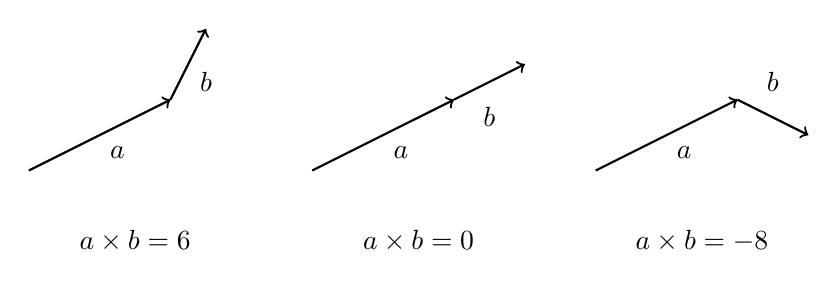
\begin{tikzpicture}[scale=0.45]

\draw[->,thick] (0,0)--(4,2);
\draw[->,thick] (4,2)--(4+1,2+2);

\node at (2.5,0.5) {$a$};
\node at (5,2.5) {$b$};

\node at (3,-2) {$a \times b = 6$};

\draw[->,thick] (8+0,0)--(8+4,2);
\draw[->,thick] (8+4,2)--(8+4+2,2+1);

\node at (8+2.5,0.5) {$a$};
\node at (8+5,1.5) {$b$};

\node at (8+3,-2) {$a \times b = 0$};

\draw[->,thick] (16+0,0)--(16+4,2);
\draw[->,thick] (16+4,2)--(16+4+2,2-1);

\node at (16+2.5,0.5) {$a$};
\node at (16+5,2.5) {$b$};

\node at (16+3,-2) {$a \times b = -8$};
\end{tikzpicture}
\end{center}

\noindent
例えば、最初のケースでは、$a=(4,2)$ and $b=(1,2)$で、次のコードは、
\texttt{complex}クラスの機能を使い、を用いて外積を計算します。

\begin{lstlisting}
P a = {4,2};
P b = {1,2};
C p = (conj(a)*b).Y; // 6
\end{lstlisting}

関数\texttt{conj}(訳註:共役複素数を得る関数)がベクトルのy座標を反転するので、
ベクトル$(x_1,-y_1)$ と $(x_2,y_2)$となり、これを掛け合わせるので、
$x_1 y_2 - x_2 y_1$となり、結果は6になります。

\subsubsection{点の位置 - Point location}

外積はある点が直線の左側にあるか右側にあるかを知るのに利用できます。
まず、線が点 $s_1$ と $s_2$ を通るとします。$s_1$ 側から $s_2$ を見て、その点を $p$ 考えます。
(訳註:どの点から見るかで左右は変わるので$s_1$からとします。)

例えば、次の図では、pは左側にあります。

\begin{center}
\begin{tikzpicture}[scale=0.45]
\draw[dashed,thick,->] (0,-3)--(12,6);
\draw[fill] (4,0) circle [radius=0.1];
\draw[fill] (8,3) circle [radius=0.1];
\draw[fill] (5,3) circle [radius=0.1];
\node at (4,-1) {$s_1$};
\node at (8,2) {$s_2$};
\node at (5,4) {$p$};
\end{tikzpicture}
\end{center}

外積$(p-s_1) \times (p-s_2)$は点$p$の位置を示します。
結果が正の場合、$p$は左側に位置し、負の場合、$p$は右側に位置し、
最後に0であれば、点$s_1$ , $s_2$ と$p$は同じ線上にある。

\subsubsection{線分の交差 - Line segment intersection}

\index{線分の交差 - line segment intersection}

次に、2つの線分$ab$と$cd$が同じあるいは交差するかを考えていきます。

\textit{Case 1:}
線分が同じ線上にあり、互いに重なり合っている場合は
この場合、交点は無限に存在するといえます。
例えば、次の図では、$c$と$b$の間の点はすべて交点である。
\begin{center}
\begin{tikzpicture}[scale=0.9]
\draw (1.5,1.5)--(6,3);
\draw (0,1)--(4.5,2.5);
\draw[fill] (0,1) circle [radius=0.05];
\node at (0,0.5) {$a$};
\draw[fill] (1.5,1.5) circle [radius=0.05];
\node at (6,2.5) {$d$};
\draw[fill] (4.5,2.5) circle [radius=0.05];
\node at (1.5,1) {$c$};
\draw[fill] (6,3) circle [radius=0.05];
\node at (4.5,2) {$b$};
\end{tikzpicture}
\end{center}

この場合、外積を用いるとすべての点が同一線上にあるかどうかを、
確認することができます。
点を並べ替えて、線分同士が重なっているかどうかを確認することができます。

\textit{Case 2:}
線分が共通の頂点を持ち、そこが唯一の交点となる場合もあります。
次の図では、交点は$b = c$です。

\begin{center}
\begin{tikzpicture}[scale=0.9]
\draw (0,0)--(4,2);
\draw (4,2)--(6,1);
\draw[fill] (0,0) circle [radius=0.05];
\draw[fill] (4,2) circle [radius=0.05];
\draw[fill] (6,1) circle [radius=0.05];

\node at (0,0.5) {$a$};
\node at (4,2.5) {$b=c$};
\node at (6,1.5) {$d$};
\end{tikzpicture}
\end{center}

この場合、交点の可能性は、$a=c$、$a=d$、$b=c$、$b=d$の4つだけ

\textit{Case 3:}
どの点でもない交差点を持つ場合。次の図では、点$p$が交点である。
\begin{center}
\begin{tikzpicture}[scale=0.9]
\draw (0,1)--(6,3);
\draw (2,4)--(4,0);
\draw[fill] (0,1) circle [radius=0.05];
\node at (0,0.5) {$c$};
\draw[fill] (6,3) circle [radius=0.05];
\node at (6,2.5) {$d$};
\draw[fill] (2,4) circle [radius=0.05];
\node at (1.5,3.5) {$a$};
\draw[fill] (4,0) circle [radius=0.05];
\node at (4,-0.4) {$b$};
\draw[fill] (3,2) circle [radius=0.05];
\node at (3,1.5) {$p$};
\end{tikzpicture}
\end{center}

点$c$と$d$が直線$ab$の異なる側にいる時、線分は正確に交差する。
これを確認するには、 外積を使えばよいです。

\subsubsection{線分から点への距離 - Point distance from a line}

また、外積の特徴として、三角形の面積を計算式で求めることができます。

\[\frac{| (a-c) \times (b-c) |}{2},\]
ここで、a,b,cは三角形の頂点の座標です。
これを用いてある点と直線の最短距離を計算する公式を導くことができます。
例えば、次の図において、点 $p$ と点$s_1$ と$s_2$ で定義される直線との最短距離を$d$ としましょう。
\begin{center}
\begin{tikzpicture}[scale=0.75]
\draw (-2,-1)--(6,3);
\draw[dashed] (1,4)--(2.40,1.2);
\node at (0,-0.5) {$s_1$};
\node at (4,1.5) {$s_2$};
\node at (0.5,4) {$p$};
\node at (2,2.7) {$d$};
\draw[fill] (0,0) circle [radius=0.05];
\draw[fill] (4,2) circle [radius=0.05];
\draw[fill] (1,4) circle [radius=0.05];
\end{tikzpicture}
\end{center}

$s_1$ ,$s_2$ ,$p$を頂点とする三角形の面積は、
$\frac{1}{2} |s_2-s_1| d$
あるいは、
$\frac{1}{2} ((s_1-p) \times (s_2-p))$
の2つの方法で計算することができます。
このため、最短の距離は、以下の通りとなります。
\[ d = \frac{(s_1-p) \times (s_2-p)}{|s_2-s_1|} .\]

\subsubsection{ポリゴン内の点 ーPoint inside a polygon}

点が多角形の内側にあるか外側にあるかを判定する問題を考えます。
例えば、次の図で点$a$は多角形の内側にあり、点$b$は多角形の外側にあるというとしましょう。

\begin{center}
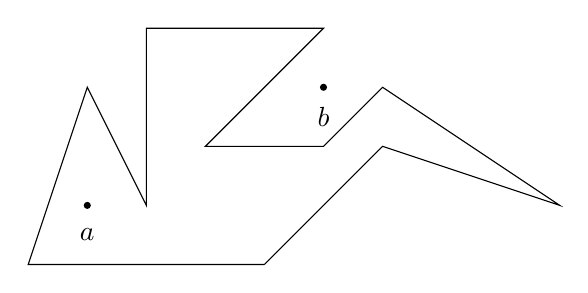
\begin{tikzpicture}[scale=0.75]
%\draw (0,0)--(2,-2)--(3,1)--(5,1)--(2,3)--(1,2)--(-1,2)--(1,4)--(-2,4)--(-2,1)--(-3,3)--(-4,0)--(0,0);
\draw (0,0)--(2,2)--(5,1)--(2,3)--(1,2)--(-1,2)--(1,4)--(-2,4)--(-2,1)--(-3,3)--(-4,0)--(0,0);

\draw[fill] (-3,1) circle [radius=0.05];
\node at (-3,0.5) {$a$};
\draw[fill] (1,3) circle [radius=0.05];
\node at (1,2.5) {$b$};
\end{tikzpicture}
\end{center}

この問題を特には興味深い方法が使えます。
点から任意の方向に光線を送り(つまり、点から十分に長い線を書く)、
それが多角形の線に触れる回数を計算します。
その回数が奇数なら、その点は多角形の内側にあり、偶数なら多角形の外側にあることが知られています。

\begin{samepage}
例を示します。
\begin{center}
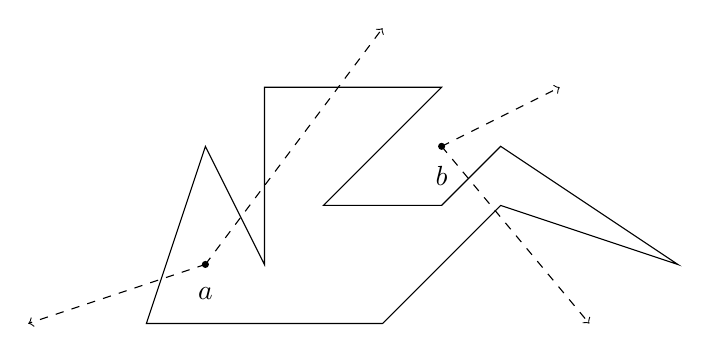
\begin{tikzpicture}[scale=0.75]
\draw (0,0)--(2,2)--(5,1)--(2,3)--(1,2)--(-1,2)--(1,4)--(-2,4)--(-2,1)--(-3,3)--(-4,0)--(0,0);

\draw[fill] (-3,1) circle [radius=0.05];
\node at (-3,0.5) {$a$};
\draw[fill] (1,3) circle [radius=0.05];
\node at (1,2.5) {$b$};

\draw[dashed,->] (-3,1)--(-6,0);
\draw[dashed,->] (-3,1)--(0,5);

\draw[dashed,->] (1,3)--(3.5,0);
\draw[dashed,->] (1,3)--(3,4);
\end{tikzpicture}
\end{center}
\end{samepage}

$a$からの光線は、ポリゴンと1回、3回接するので、$a$はポリゴンの内側にあることになります。
これに対応して$b$からの光線はポリゴンの境界と0回と2回接するので、$b$ はポリゴンの外側にあることになります。

\section{ポリゴンの面積 - Polygon area}

多角形の面積を計算するための一般的な公式は
\key{靴紐アルゴリズム - shoelace formula}と呼ばれ、以下のように示されます。
\index{靴紐アルゴリズム - shoelace formula}

\[\frac{1}{2} |\sum_{i=1}^{n-1} (p_i \times p_{i+1})| =
\frac{1}{2} |\sum_{i=1}^{n-1} (x_i y_{i+1} - x_{i+1} y_i)|, \]
ここで,頂点は,$p_1=(x_1,y_1)$, $p_2=(x_2,y_2)$, $\ldots$, $p_n=(x_n,y_n)$
,$p_i$と$p_{i+1}$ が多角形の境界で隣接し,
最初と最後の頂点が同じになる順序,つまり  $p_1=p_n$ とします。

例えば、
\begin{center}
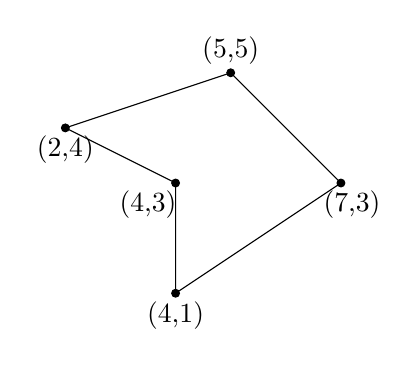
\begin{tikzpicture}[scale=0.7]
\filldraw (4,1.4) circle (2pt);
\filldraw (7,3.4) circle (2pt);
\filldraw (5,5.4) circle (2pt);
\filldraw (2,4.4) circle (2pt);
\filldraw (4,3.4) circle (2pt);
\node (1) at (4,1) {(4,1)};
\node (2) at (7.2,3) {(7,3)};
\node (3) at (5,5.8) {(5,5)};
\node (4) at (2,4) {(2,4)};
\node (5) at (3.5,3) {(4,3)};
\path[draw] (4,1.4) -- (7,3.4) -- (5,5.4) -- (2,4.4) -- (4,3.4) -- (4,1.4);
\end{tikzpicture}
\end{center}

このポリゴンの面積の面積は以下の通りです。
\[\frac{|(2\cdot5-5\cdot4)+(5\cdot3-7\cdot5)+(7\cdot1-4\cdot3)+(4\cdot3-4\cdot1)+(4\cdot4-2\cdot3)|}{2} = 17/2.\]

この考え方は$y$軸を一辺にもち、もう一方をポリゴンの辺に持つ台形を用いて面積を求めていきます。
\begin{center}
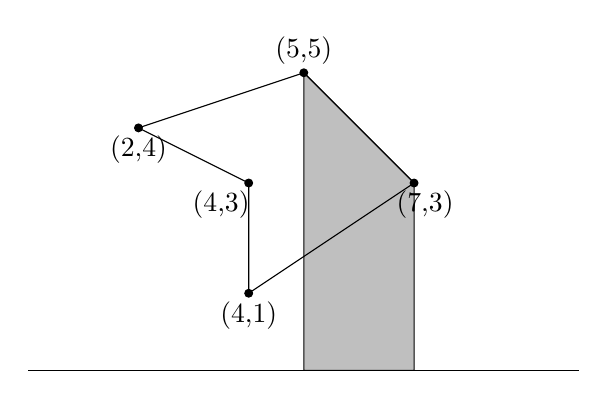
\begin{tikzpicture}[scale=0.7]
\path[draw,fill=lightgray] (5,5.4) -- (7,3.4) -- (7,0) -- (5,0) -- (5,5.4);
\filldraw (4,1.4) circle (2pt);
\filldraw (7,3.4) circle (2pt);
\filldraw (5,5.4) circle (2pt);
\filldraw (2,4.4) circle (2pt);
\filldraw (4,3.4) circle (2pt);
\node (1) at (4,1) {(4,1)};
\node (2) at (7.2,3) {(7,3)};
\node (3) at (5,5.8) {(5,5)};
\node (4) at (2,4) {(2,4)};
\node (5) at (3.5,3) {(4,3)};
\path[draw] (4,1.4) -- (7,3.4) -- (5,5.4) -- (2,4.4) -- (4,3.4) -- (4,1.4);
\draw (0,0) -- (10,0);
\end{tikzpicture}
\end{center}
このような台形の面積は、$p_i$ と $p_{i+1}$に注目した時、
\[(x_{i+1}-x_{i}) \frac{y_i+y_{i+1}}{2},\]
となります。さて、先ほどのルールに従い点は並んでいるため、
$x_{i+1}>x_{i}$である時、この面積は加算すべきで、
$x_{i+1}<x_{i}$であるとき、面積は減算すべきです。

このようにポリゴンの面積を台形の面積で求めることができました。
\[|\sum_{i=1}^{n-1} (x_{i+1}-x_{i}) \frac{y_i+y_{i+1}}{2}| =
\frac{1}{2} |\sum_{i=1}^{n-1} (x_i y_{i+1} - x_{i+1} y_i)|.\]

ポリゴンの境界に沿って時計回りに走査するか反時計回りに走査するかによって、
和の値が正または負になることがあるので、和の絶対値をとることに注意してください。

\subsubsection{ピックの定理 - Pick's theorem}

\index{ピックの定理 - Pick's theorem}

\key{ピックの定理 - Pick's theorem} は、多角形のすべての頂点が整数の座標を持つ場合に、
多角形の面積を計算する方法を提供します。
ピックの定理によれば、多角形の面積で示すことができます。
\[ a + b/2 -1,\]
ここで、$a$はポリゴン内部の整数点の数、$b$はポリゴンの境界上の整数点の数です。

例えば、ポリゴンの面積
\begin{center}
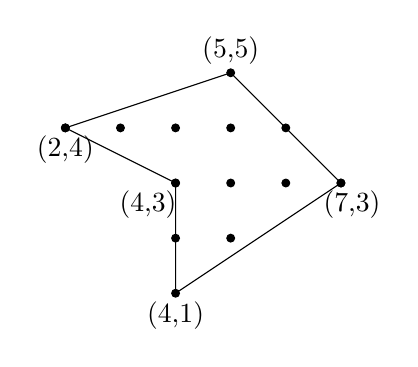
\begin{tikzpicture}[scale=0.7]
\filldraw (4,1.4) circle (2pt);
\filldraw (7,3.4) circle (2pt);
\filldraw (5,5.4) circle (2pt);
\filldraw (2,4.4) circle (2pt);
\filldraw (4,3.4) circle (2pt);
\node (1) at (4,1) {(4,1)};
\node (2) at (7.2,3) {(7,3)};
\node (3) at (5,5.8) {(5,5)};
\node (4) at (2,4) {(2,4)};
\node (5) at (3.5,3) {(4,3)};
\path[draw] (4,1.4) -- (7,3.4) -- (5,5.4) -- (2,4.4) -- (4,3.4) -- (4,1.4);

\filldraw (2,4.4) circle (2pt);
\filldraw (3,4.4) circle (2pt);
\filldraw (4,4.4) circle (2pt);
\filldraw (5,4.4) circle (2pt);
\filldraw (6,4.4) circle (2pt);

\filldraw (4,3.4) circle (2pt);
\filldraw (5,3.4) circle (2pt);
\filldraw (6,3.4) circle (2pt);
\filldraw (7,3.4) circle (2pt);

\filldraw (4,2.4) circle (2pt);
\filldraw (5,2.4) circle (2pt);
\end{tikzpicture}
\end{center}
は$6+7/2-1=17/2$となります。

\section{距離関数 - Distance functions}

\index{距離関数 - distance function}
\index{ユークリッド距離 - Euclidean distance}
\index{マンハッタン距離 - Manhattan distance}

\key{距離関数 - distance function}は2点の距離を求める関数です。
一般的な距離は
\key{ユークリッド距離 - Euclidean distance} で、 
$(x_1,y_1)$ と $(x_2,y_2)$ に対して以下のように定まります。
\[\sqrt{(x_2-x_1)^2+(y_2-y_1)^2}.\]
時に、
\key{マンハッタン距離 - Manhattan distance}
も使われ、これは以下のように示されます。
\[|x_1-x_2|+|y_1-y_2|.\]
\begin{samepage}
次のように絵で考えてみます。
\begin{center}
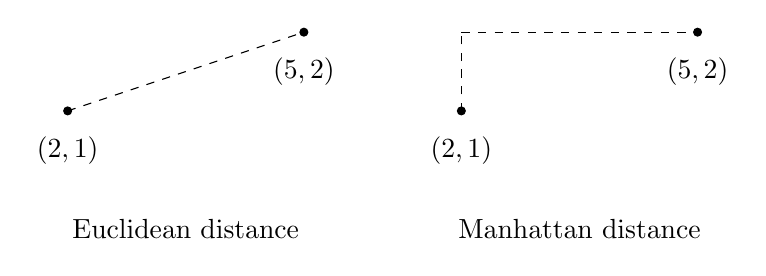
\begin{tikzpicture}

\draw[fill] (2,1) circle [radius=0.05];
\draw[fill] (5,2) circle [radius=0.05];

\node at (2,0.5) {$(2,1)$};
\node at (5,1.5) {$(5,2)$};

\draw[dashed] (2,1) -- (5,2);

\draw[fill] (5+2,1) circle [radius=0.05];
\draw[fill] (5+5,2) circle [radius=0.05];

\node at (5+2,0.5) {$(2,1)$};
\node at (5+5,1.5) {$(5,2)$};

\draw[dashed] (5+2,1) -- (5+2,2);
\draw[dashed] (5+2,2) -- (5+5,2);

\node at (3.5,-0.5) {Euclidean distance};
\node at (5+3.5,-0.5) {Manhattan distance};
\end{tikzpicture}
\end{center}
\end{samepage}
ユークリッド距離は、
\[\sqrt{(5-2)^2+(2-1)^2}=\sqrt{10}\]
となり、マンハッタン距離は
\[|5-2|+|2-1|=4.\]
となります。
次の図は、ユークリッド距離とマンハッタン距離を用いた
中心点から1以内の 距離にある領域です。
\begin{center}
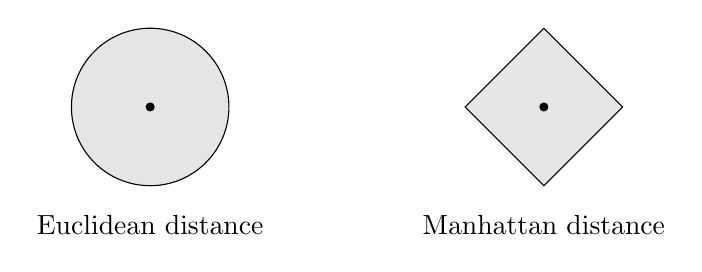
\begin{tikzpicture}

\draw[fill=gray!20] (0,0) circle [radius=1];
\draw[fill] (0,0) circle [radius=0.05];

\node at (0,-1.5) {Euclidean distance};

\draw[fill=gray!20] (5+0,1) -- (5-1,0) -- (5+0,-1) -- (5+1,0) -- (5+0,1);
\draw[fill] (5,0) circle [radius=0.05];
\node at (5,-1.5) {Manhattan distance};
\end{tikzpicture}
\end{center}

\subsubsection{回転座標 - Rotating coordinates}

ユークリッド距離の代わりにマンハッタン距離を使うと解きやすくなる問題もあります。
例として、2次元平面上の$n$個の点が与えられ、
任意の2点間の最大マンハッタン距離を計算する問題を考えてみます。

例えば、次のような点の集合があったとしましょう。
\begin{center}
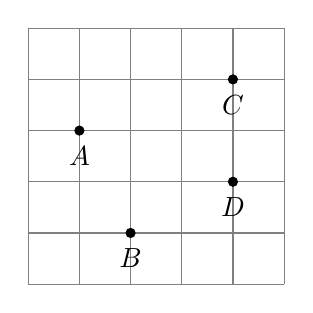
\begin{tikzpicture}[scale=0.65]
\draw[color=gray] (-1,-1) grid (4,4);

\filldraw (0,2) circle (2.5pt);
\filldraw (3,3) circle (2.5pt);
\filldraw (1,0) circle (2.5pt);
\filldraw (3,1) circle (2.5pt);

\node at (0,1.5) {$A$};
\node at (3,2.5) {$C$};
\node at (1,-0.5) {$B$};
\node at (3,0.5) {$D$};
\end{tikzpicture}
\end{center}
ここでのマンハッタン距離の最大値は$B$と$C$の$5$です。
\begin{center}
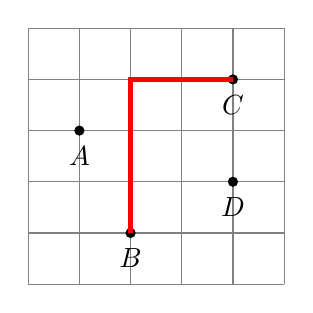
\begin{tikzpicture}[scale=0.65]
\draw[color=gray] (-1,-1) grid (4,4);

\filldraw (0,2) circle (2.5pt);
\filldraw (3,3) circle (2.5pt);
\filldraw (1,0) circle (2.5pt);
\filldraw (3,1) circle (2.5pt);

\node at (0,1.5) {$A$};
\node at (3,2.5) {$C$};
\node at (1,-0.5) {$B$};
\node at (3,0.5) {$D$};

\path[draw=red,thick,line width=2pt] (1,0) -- (1,3) -- (3,3);
\end{tikzpicture}
\end{center}


マンハッタン距離を用いた便利なテクニックは、点$(x, y)$が、
$(x + y, y - x)$になる ように、
すべての座標を45度回転させることです。
例えば、上記の点を回転させた結果は、以下のようになります。

\begin{center}
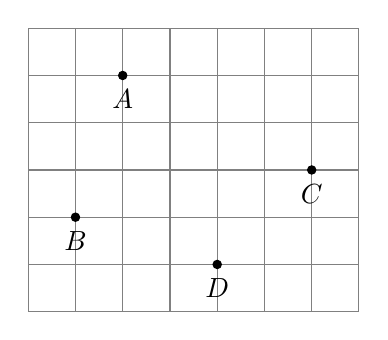
\begin{tikzpicture}[scale=0.6]
\draw[color=gray] (0,-3) grid (7,3);

\filldraw (2,2) circle (2.5pt);
\filldraw (6,0) circle (2.5pt);
\filldraw (1,-1) circle (2.5pt);
\filldraw (4,-2) circle (2.5pt);

\node at (2,1.5) {$A$};
\node at (6,-0.5) {$C$};
\node at (1,-1.5) {$B$};
\node at (4,-2.5) {$D$};
\end{tikzpicture}
\end{center}
最大の距離は以下のようになります。
\begin{center}
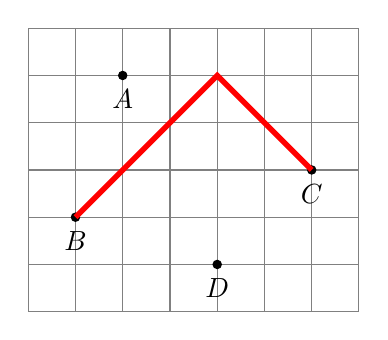
\begin{tikzpicture}[scale=0.6]
\draw[color=gray] (0,-3) grid (7,3);

\filldraw (2,2) circle (2.5pt);
\filldraw (6,0) circle (2.5pt);
\filldraw (1,-1) circle (2.5pt);
\filldraw (4,-2) circle (2.5pt);

\node at (2,1.5) {$A$};
\node at (6,-0.5) {$C$};
\node at (1,-1.5) {$B$};
\node at (4,-2.5) {$D$};

\path[draw=red,thick,line width=2pt] (1,-1) -- (4,2) -- (6,0);
\end{tikzpicture}
\end{center}

回転座標がp!1=(x1!,y1!)とp!2=(x2!,y2!)である2点p1 =(x1 ,y1 )とp2 = (x2 , y2 ) を考えよう。ここで、p1 と p2 の間の Manhat- tan 距離を表現する方法は
2つあります。
ここで、2つの点$p_1=(x_1,y_1)$ と $p_2=(x_2,y_2)$ を回転させた座標である
$p'_1=(x'_1,y'_1)$ と
$p'_2=(x'_2,y'_2)$を考えます。
今、$p_1$ と $p_2$のマンハッタン距離は2つの方法で表現できます。
\[|x_1-x_2|+|y_1-y_2| = \max(|x'_1-x'_2|,|y'_1-y'_2|)\]

例えば、$p_1=(1,0)$ と $p_2=(3,3)$の場合、
回転した座標は $p'_1=(1,-1)$ と $p'_2=(6,0)$
であり、マンハッタン距離は、次の通りです。
\[|1-3|+|0-3| = \max(|1-6|,|-1-0|) = 5.\]

回転座標は、xとyの座標を別々に考えることができるため、
マンハッタン距離の操作は簡単に行うことができます。
2点間のマンハッタン距離を最大にするには、
回転座標の値が最大となる2点を見つければよいです。
\[\max(|x'_1-x'_2|,|y'_1-y'_2|).\]
これは簡単に求められ、回転した座標の水平または垂直方向の差のどちらかが最大であればよいからです。